\icode{N17S-ME-CA-L3-260625-001}
\nceeID[16]{2017江苏}{22}
如图所示，两个半圆柱\(A\)、\(B\)紧靠着静置于水平地面上，其上有一光滑圆柱\(C\)，三者半径均为\(R\)。\(C\)的质量为\(m\)，\(A\)、\(B\)的质量都为\(\frac{m}{2}\)，与地面的动摩擦因数均为\(\mu\)。现用水平向右的力拉\(A\)，使\(A\)缓慢移动，直至\(C\)恰好降到地面。整个过程中\(B\)保持静止。设最大静摩擦力等于滑动摩擦力，重力加速度为\(g\)。求：
\begin{enumerate}
	\item 未拉\(A\)时，\(C\)受到\(B\)作用力的大小\(F\)；
	\item 动摩擦因数的最小值\(\mu_{\mathrm{min}}\)；
	\item \(A\)移动的整个过程中，拉力做的功\(W\)。
\end{enumerate}
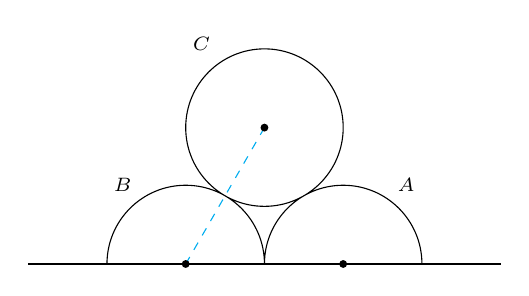
\begin{tikzpicture}[font=\scriptsize]
	\draw (0,0) arc(0:180:1) (2,0) arc(0:180:1) (0,{sqrt(3)})circle(1);
	\draw (-3,0)--(3,0);
	\draw[dashed,cyan] (0,{sqrt(3)})--(-1,0);
	\fill (-1,0) circle(.05) (1,0) circle(.05) (0,{sqrt(3)}) circle(.05);
	\node at(-1.8,1){\(B\)};
	\node at(1.8,1){\(A\)};
	\node at(-.8,2.8){\(C\)};
\end{tikzpicture}
\begin{answer}
	（1）\(F = \frac{\sqrt{3}}{3}mg\)（2）\(\mu_{\min} = \frac{\sqrt{3}}{2}\)（3）\(W = (2\mu - 1)(\sqrt{3} - 1)mgR\)\qquad 提示：\(A\)、\(C\)缓慢移动，则动能为0，地面对\(A\)的摩擦力是恒力\(f = \mu mg\)，可得：\(W + mg\cdot(\sqrt{3}R - R) - \mu mg\cdot(2 \sqrt{3}R - 2R) = 0\)

	\begin{tikzpicture}[>=stealth,font=\scriptsize]
	\draw[gray] (0,0) arc(0:180:1) (2,0) arc(0:180:1) (0,{sqrt(3)})circle(1)coordinate(o) (-3,0)--(3,0);
	\draw[dashed,cyan] (1,0)--(0,{sqrt(3)})--(-1,0);
	\fill (-1,0) circle(.05) (1,0) circle(.05) (0,{sqrt(3)}) circle(.05);
	\draw[dashed,gray] ($(o)+(120:.8)$)--++(60:.8)--++(-60:.8);
	\draw[->,blue] (o)--++(60:.8);
	\draw[->,blue] (o)--++(120:.8);
	\draw[->,red] (o)--++(0,{-.8*sqrt(3)});
	\draw[->,dashed,red] (o)--++(0,{.8*sqrt(3)});
	\node at(0,-1.2){图甲};
	\end{tikzpicture}
	\begin{tikzpicture}[>=stealth,font=\scriptsize]
	\draw[gray] (0,0) arc(0:180:1) ({2*sqrt(3)},0) arc(0:180:1) ({sqrt(3)-1},1)circle(1)coordinate(o) (-3,0)--(4,0);
	\draw[dashed,cyan] ({2*sqrt(3)-1},0)--(o)--(-1,0) (o)--++(0,-1);
	\fill (-1,0) circle(.05) ({2*sqrt(3)-1},0) circle(.05) (o) circle(.05);
	\draw[->,blue] (-1,0)--++(-150:1.6)node[below left,black]{\(N_1\)};
	\draw[->,teal] (-1,0)--++(0,-.8)node[right,black]{\(\frac{1}{2}mg\)};
	\draw[->,red] (-1,0)--++({.8*sqrt(3)},0)node[below,black]{\(f\)};
	\draw[->,magenta] (-1,0)--++(0,1.6)node[left,black]{\(N\)};
	\node at({sqrt(3)-1},-1.2){图乙};
	\end{tikzpicture}
\end{answer}